\documentclass[12pt,a4paper]{article}

\usepackage[utf8]{inputenc}
\usepackage[margin=2.5cm]{geometry}
\usepackage{amsmath, amssymb}
\usepackage{graphicx}
\usepackage{listings}
\usepackage{xcolor}
\usepackage{hyperref}
\usepackage{float}

\lstset{
    language=Python,
    basicstyle=\ttfamily\small,
    keywordstyle=\color{blue},
    commentstyle=\color{gray},
    stringstyle=\color{red},
    numbers=left,
    numberstyle=\tiny\color{gray},
    frame=single,
    breaklines=true,
    captionpos=b
}

\title{Spectral-Domain Bayesian Audio Signal Processing}
\author{Reilly}
\date{March 2026}

\begin{document}

\maketitle

\begin{abstract}
This report documents the development of a spectral-domain Bayesian approach to audio signal denoising and source separation. The project implements Wiener filtering with learned priors in the Short-Time Fourier Transform (STFT) domain. We begin with fundamental signal generation and spectral analysis, building toward a full Bayesian denoising pipeline.
\end{abstract}

\tableofcontents
\newpage

\section{Introduction}

The goal of this project is to implement a Bayesian framework for audio signal processing that operates in the spectral domain. The core technique is Wiener filtering, where the optimal filter gain at each time-frequency bin is determined by estimates of the signal and noise power spectral densities (PSDs). By placing priors on these PSDs, we obtain a principled, probabilistic approach to denoising and source separation.

\section{Signal Generation and Spectral Analysis}

\subsection{Composite Signal Generation}

We begin by constructing a test signal composed of multiple sinusoidal components. The signal is defined as a sum of sinusoids:

\begin{equation}
    x(t) = \sum_{i} A_i \sin(2\pi f_i t + \phi_i)
\end{equation}

where $A_i$, $f_i$, and $\phi_i$ are the amplitude, frequency, and random phase offset of each component. The random phase ensures a more realistic signal that does not start with all components aligned at zero. Our test signal uses three components:

\begin{center}
\begin{tabular}{cccc}
    \hline
    Component & Amplitude & Frequency (Hz) & Phase \\
    \hline
    1 & 0.67 & 320 & $\phi_1 \sim \mathcal{U}(0, 2\pi)$ \\
    2 & 0.74 & 240 & $\phi_2 \sim \mathcal{U}(0, 2\pi)$ \\
    3 & 1.00 & 160 & $\phi_3 \sim \mathcal{U}(0, 2\pi)$ \\
    \hline
\end{tabular}
\end{center}

The signal is sampled at $f_s = 15000$ Hz over a duration of 0.1 seconds, producing $N = 1500$ samples.

\begin{figure}[H]
    \centering
    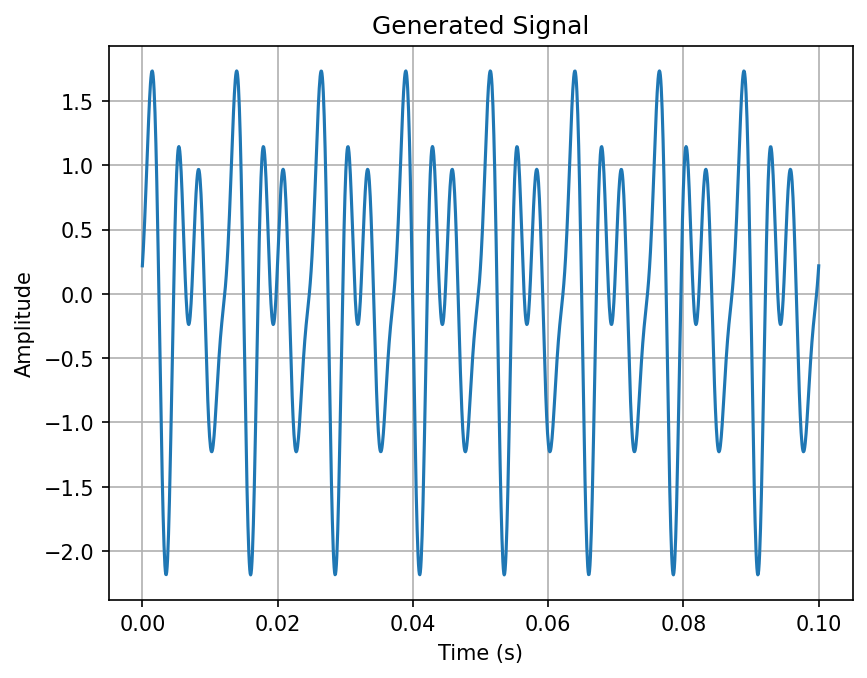
\includegraphics[width=\textwidth]{figures/signal.png}
    \caption{Time-domain representation of the composite test signal.}
    \label{fig:signal}
\end{figure}

\subsection{The Discrete Fourier Transform}

To analyse the frequency content of the signal, we implement the Discrete Fourier Transform (DFT) directly from its definition:

\begin{equation}
    X[k] = \sum_{n=0}^{N-1} x[n] \, e^{-j 2\pi k n / N}, \quad k = 0, 1, \ldots, N-1
\end{equation}

Rather than using nested loops, the implementation vectorises this computation using NumPy broadcasting. The indices $k$ and $n$ are formed as a column vector and row vector respectively, producing the full $N \times N$ twiddle factor matrix in a single operation:

\begin{lstlisting}[caption={Vectorised DFT implementation}]
def DFT(x):
    N = len(x)
    n = np.arange(N)
    k = np.arange(N).reshape(-1, 1)
    X = np.sum(x * np.exp(-2j * np.pi * k * n / N), axis=1)
    return X
\end{lstlisting}

\subsection{Frequency Spectrum Visualisation}

The magnitude spectrum is computed as $|X[k]| / N$ and displayed as a bar chart over the single-sided frequency range $[0, f_s/2)$. The frequency axis is automatically scaled to focus on bins with significant energy, defined as those exceeding 1\% of the peak magnitude.

The three frequency components at 160, 240, and 320 Hz are clearly resolved in the resulting spectrum, with magnitudes proportional to their respective amplitudes.

\begin{figure}[H]
    \centering
    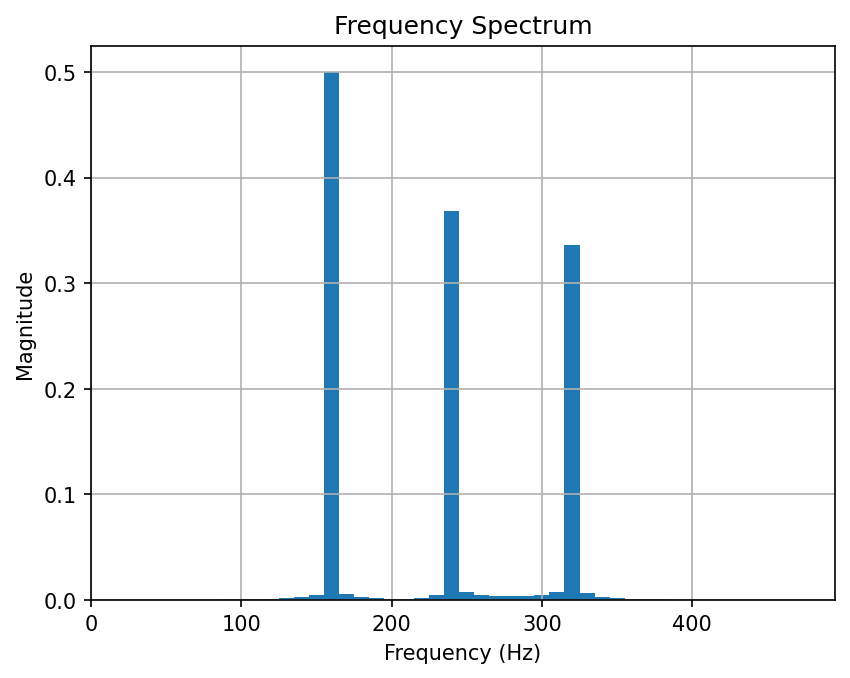
\includegraphics[width=\textwidth]{figures/spectrum.png}
    \caption{Single-sided magnitude spectrum of the test signal, showing peaks at 1, 2, and 10 Hz.}
    \label{fig:spectrum}
\end{figure}

\section{Next Steps}

The following stages of the project will build on this spectral analysis foundation:

\begin{enumerate}
    \item \textbf{STFT implementation} --- windowed, overlapping spectral analysis for time-varying signals.
    \item \textbf{Wiener filter} --- optimal spectral-domain gain computation given signal and noise PSD estimates.
    \item \textbf{Noise prior models} --- stationary, adaptive, and NMF-based prior estimation.
    \item \textbf{Variational inference} --- full Bayesian treatment with uncertainty quantification.
    \item \textbf{Source separation} --- multi-source Wiener filtering for mixed audio signals.
\end{enumerate}

\end{document}
